\centering
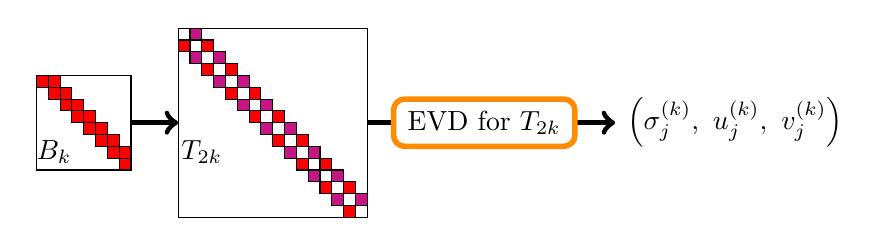
\begin{tikzpicture}[scale=.3]
  \pgfmathsetmacro{\ix}{1}
  \pgfmathsetmacro{\isx}{.5}
  %% \begin{scope}
  %%   \draw[fill=white] (0,-2) rectangle +(4,4);
  %%   \foreach \x in { 0,...,3 }
  %%   \draw[fill=ForestGreen] (\x*\ix+\ix,2-\ix-\x*\ix) -- (\x*\ix+\ix,2-\ix-\x*\ix+\ix) -- (\x*\ix,2-\ix-\x*\ix+\ix) -- cycle;
  %%   \foreach \x in { 1,...,3 }
  %%   \draw[fill=ForestGreen] (\x*\ix+\ix,2-\x*\ix) -- (\x*\ix,2-\x*\ix) -- (\x*\ix,2-\x*\ix+\ix) -- cycle;
  %%   \draw (0.75,-1.25) node{$\overline{B}_k$};
  %% \end{scope}

  %% \begin{scope}[shift={(0:4)}]
  %%   \draw [->,thick,line width=2pt] (0,0) -- (2,0);
  %% \end{scope}

  \begin{scope}[shift={(0:0)}]
    \draw[fill=white] (0,-2) rectangle +(4,4);
    \foreach \x in { 0,...,7 }
    \draw[fill=red] (\x*\isx,2-\isx-\x*\isx) rectangle +(\isx,\isx);
    \foreach \x in { 0,...,6 }
    \draw[fill=red] (\x*\isx+\isx,2-\isx-\x*\isx) rectangle +(\isx,\isx);
    %% \foreach \x in { 0,...,6 }
    %% \draw[fill=red] (\x*\ix,2-2*\ix-\x*\ix) rectangle +(\ix,\ix);
    \draw (0.75,-1.25) node{$B_k$};
  \end{scope}

  \begin{scope}[shift={(0:4)}]
    \draw [->,thick,line width=2pt] (0,0) -- (2,0);
  \end{scope}

  \begin{scope}[shift={(0:6)}]
    \draw[fill=white] (0,-4) rectangle +(8,8);
    \foreach \x in { 1,...,7 }
    \draw[fill=red] (2*\x*\isx,4-2*\x*\isx) rectangle +(\isx,\isx);
    \foreach \x in { 0,...,7 }
    \draw[fill=red] (2*\x*\isx,4-2*\isx-2*\x*\isx) rectangle +(\isx,\isx);
    \foreach \x in { 0,...,7 }
    \draw[fill=MediumVioletRed] (2*\x*\isx+\isx,4-\isx-2*\x*\isx) rectangle +(\isx,\isx);
    \foreach \x in { 1,...,7 }
    \draw[fill=MediumVioletRed] (2*\x*\isx-\isx,4-2*\x*\isx-\isx) rectangle +(\isx,\isx);
    \draw (1,-1.25) node{$T_{2k}$};
  \end{scope}

  \begin{scope}[shift={(0:14)}]
    \draw [->,thick,line width=2pt] (0,0) --
    (1,0) node[right,align=center, text width=2cm,rounded corners,draw=DarkOrange,fill=white,inner sep=1ex]{EVD for $T_{2k}$} --
    (10.5,0) node[right,align=center]{$\left(\sigma^{(k)}_j,\ \bm{u}^{(k)}_j,\ \bm{v}^{(k)}_j\right)$};
  \end{scope}
\end{tikzpicture}
